\documentclass[12pt,compress,aspectratio=169]{beamer}
\usetheme{metropolis}
\setbeamersize{text margin left=.5cm,text margin right=.5cm}
%\usefonttheme{professionalfonts}
\usepackage[lf]{carlito}
\usepackage{siunitx}
\usepackage{tikz}
\usepackage{mathpazo}
\usepackage{bm}
%\usepackage{xcolor,colortbl}

\usetikzlibrary{patterns}

%\setmonofont{Ubuntu Mono}
\setlength{\parskip}{0pt}
\setlength{\itemsep}{0pt}
\renewcommand{\baselinestretch}{1}

\sisetup{
  inter-unit-product=\cdotp,
  per-mode=symbol
}
\tikzset{>=latex}

\title{Topic 6: Circular Motion}
\subtitle{Advanced Placement Physics C}
\author[TML]{Dr.\ Timothy Leung}
\institute{Olympiads School}
\date{\today}

\newcommand{\pic}[2]{\includegraphics[width=#1\textwidth]{#2}}
\newcommand{\eq}[2]{\vspace{#1}{\Large\begin{displaymath}#2\end{displaymath}}}


\begin{document}

\begin{frame}
  \maketitle
\end{frame}


%\begin{frame}{Files to Download}
%  Please download the following files from the school website if you have not
%  already done so:
%  \begin{itemize}
%  \item\texttt{PhysAPC-06-circMotion.pdf}---The ``print version'' of the
%    class slides for this topic.
%  \item\texttt{PhysAPC-06-Homework.pdf}---Homework problems for this topic.
%  \end{itemize}
%  \vspace{.1in}Please download/print the PDF file for the class slides before
%  each class. There is no point copying notes that are already on the slides.
%  Instead, focus on things that aren't necessarily on the slides. If you wish
%  to print the slides, we recommend printing 4 slides per page.
%\end{frame}



\begin{frame}{Review of Circular Motion}
  In a \textbf{circular motion}, an object of mass $m$ moves in a circular path
  about a fixed center. In Grade 12 Physics, you should have studied
  \emph{uniform} circular motion, where:
  \begin{itemize}
  \item the object's speed (magnitude of velocity) is constant
  \item the object's \textbf{centripetal acceleration} is toward the center
  \item the object's acceleration is caused by a \textbf{centripetal force}
  \end{itemize}
\end{frame}



\section{Polar Coordinates}

\begin{frame}{Polar Coordinate System in 2D}
  \begin{columns}
    \column{.32\textwidth}
    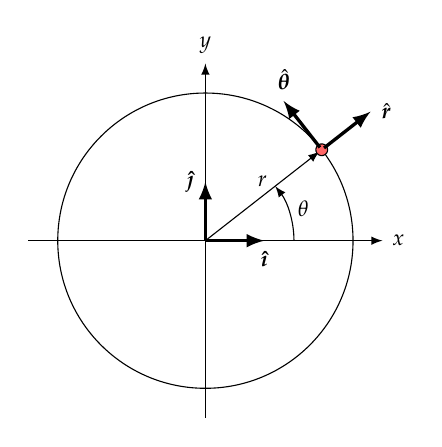
\begin{tikzpicture}[scale=.75]
      \begin{scope}[->]
        \draw(-3,0)--(3,0) node[right]{\footnotesize$x$};
        \draw(0,-3)--(0,3) node[above]{\footnotesize$y$};
      \end{scope}
      \begin{scope}[very thick,->]
        \draw(0,0)--(1,0) node[below]{\footnotesize$\bm{\hat{\imath}}$};
        \draw(0,0)--(0,1) node[left]{\footnotesize$\bm{\hat{\jmath}}$};
      \end{scope}
      \draw (0,0) circle(2.5);
      \begin{scope}[rotate=38]
        \draw[->] (0,0)--(2.45,0) node[midway,above]{\footnotesize$r$};
        \draw[fill=red!60] (2.5,0) circle(.1);
        \begin{scope}[very thick,->]
          \draw(2.55,0)--(3.55,0) node[right]{\footnotesize$\hat{\bm{r}}$};
          \draw(2.5,.05)--(2.5,1.05)
          node[above]{\footnotesize$\hat{\bm{\theta}}$};
          \end{scope}
      \end{scope}
      \draw(1.5,0)[->] arc(0:38:1.5) node[pos=.55,right]{\footnotesize$\theta$};
    \end{tikzpicture}

    \column{.68\textwidth}
    In the Cartesian coordinate system, an object's position is described by
    its $x$ and $y$ coordinates:

    \eq{-.25in}{
      \bm{x}(t)=x(t)\bm{\hat{\imath}} + y(t) \bm{\hat{\jmath}}
      }

    \vspace{-.15in}For circular motion or general rotational motion, the
    \textbf{polar coordinate system} is preferred. The position of an object
    is described by:

    \eq{-.2in}{
      \bm{r}(t)=r(t)\hat{\bm{r}} + \theta(t)\hat{\bm{\theta}}
    }
    \begin{itemize}
    \item\vspace{-.15in}$r$ is distance from the origin
    \item $\theta$ is the standard angle, measured counter clockwise from the
      $x$ axis in \emph{radians}
    \end{itemize}
  \end{columns}
\end{frame}



\begin{frame}{Polar Coordinate System in 2D}
  \begin{columns}
    \column{.3\textwidth}
    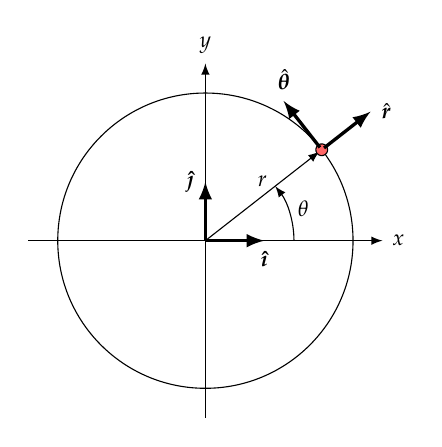
\begin{tikzpicture}[scale=.75]
      \draw[->](-3,0)--(3,0) node[right]{\footnotesize$x$};
      \draw[->](0,-3)--(0,3) node[above]{\footnotesize$y$};
      \draw[very thick,->](0,0)--(1,0)
      node[below]{\footnotesize$\bm{\hat{\imath}}$};
      \draw[very thick,->](0,0)--(0,1)
      node[left]{\footnotesize$\bm{\hat{\jmath}}$};
      \draw (0,0) circle(2.5);
      \begin{scope}[rotate=38]
        \draw[->] (0,0)--(2.45,0) node[midway,above]{\footnotesize$r$};
        \draw[fill=red!60] (2.5,0) circle(.1);
        \draw[very thick,->](2.55,0)--(3.55,0)
        node[right]{\footnotesize$\hat{\bm{r}}$};
        \draw[very thick,->](2.5,.05)--(2.5,1.05)
        node[above]{\footnotesize$\hat{\bm{\theta}}$};        
      \end{scope}
      \draw(1.5,0)[->] arc(0:38:1.5) node[pos=.55,right]{\footnotesize$\theta$};
    \end{tikzpicture}

    \column{.7\textwidth}
    \begin{itemize}
    \item Like the Cartesian system, the polar coordinate system is also
      right-handed
    \item Both basic vectors $\hat{\bm{r}}$ (radial direction) and
      $\hat{\bm{\theta}}$ (angular direction) rotate as the object moves
    \item Simpler way is to think of position as just two
      parameters, which is \emph{exactly} how position vectors are expressed in
      Grade 11/12 Physics: magnitude ($r$) and direction ($\theta$)!
    \item Cartesian and polar coordinates are related by:
      
      \vspace{-.35in}{\large
        \begin{align*}
          x&=r\cos\theta\\
          y&=r\sin\theta
        \end{align*}
      }
    \end{itemize}
  \end{columns}
\end{frame}



\begin{frame}{Cylindrical Coordinates in 3D}
  \begin{columns}
    \column{.45\textwidth}
    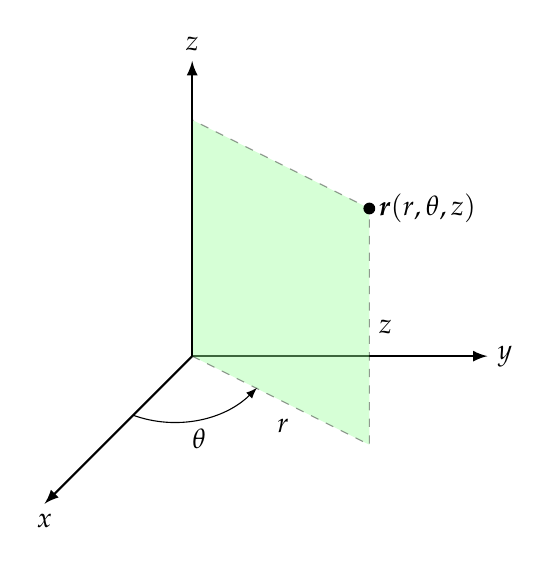
\begin{tikzpicture}[scale=.75]
      \draw[thick,->](0,0)--(-2.5,-2.5)node[below]{$x$};
      \draw[thick,->](0,0)--(5,0)   node[right]{$y$};
      \draw[dashed,fill=green!40,opacity=.4](0,0)--(3,-1.5)
      node[pos=.6,below left,opacity=1]{$r$}--(3,2.5)
      node[midway,right,black,opacity=1]{$z$}--(0,4);
      \fill[black](3,2.5) circle(.1) node[right]{$\bm{r}(r,\theta,z)$};
      \draw[->] (-1,-1) arc(-110:-45:2) node[midway,below]{$\theta$};
      \draw[thick,->](0,0)--(0,5) node[above]{$z$};
    \end{tikzpicture}

    \column{.55\textwidth}
    One way to extend the coordinates coordinate system into 3D is the
    \textbf{cylindrical coordinate system}. Note that the discussions for this
    topic focuses on $xy$ plane. Since the $z$-axis is linearly independent of
    the $xy$ plane, motion along that direction is independent.
  \end{columns}
\end{frame}



\section{Rigid-Body Circular Motion}

\begin{frame}{Angular Position and Angular Velocity}
  \vspace{.2in}
  \begin{columns}
    \column{.32\textwidth}
    \begin{tikzpicture}[scale=.75]
      \draw[->](-3,0)--(3,0) node[right]{\footnotesize$x$};
      \draw[->](0,-3)--(0,3) node[above]{\footnotesize$y$};
      \draw (0,0) circle(2.5);
      \begin{scope}[rotate=38]
        \draw[->] (0,0)--(2.44,0) node[midway,above]{\footnotesize$r$};
        \draw[fill=red!60] (2.5,0) circle(.1);
      \end{scope}
      \draw(1,0)[->] arc(0:38:1) node[midway,right]{\footnotesize$\theta$};
    \end{tikzpicture}
    
    \column{.68\textwidth}
    For a constant $r$, the \textbf{angular position} $\theta$ determines an
    object's position as a function of time:
      
    \eq{-.2in}{
      \boxed{\theta=\theta(t)}
    }
    
    \textbf{Angular velocity} $\omega$ (or \textbf{angular frequency}) is its
    time derivative:
      
    \eq{-.2in}{
      \boxed{\omega(t)=\frac{d\theta(t)}{dt}=\dot{\theta}}
    }

    $\theta$ is measured in \si{radians}, and $\omega$ in \si{rad/\s}
  \end{columns}
\end{frame}



\begin{frame}{Velocity and Angular Velocity}
  \begin{columns}
    \column{.35\textwidth}
    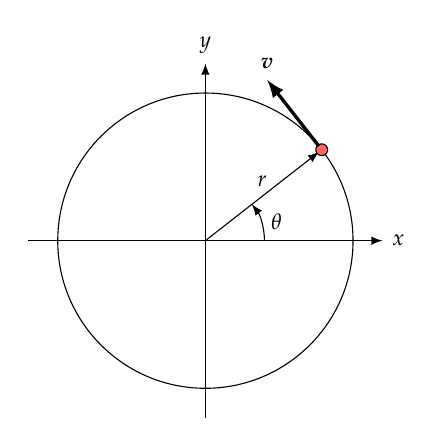
\begin{tikzpicture}[scale=.75]
      \draw[->](-3,0)--(3,0) node[right]{\footnotesize$x$};
      \draw[->](0,-3)--(0,3) node[above]{\footnotesize$y$};
      \draw (0,0) circle(2.5);
      \begin{scope}[rotate=38]
        \draw[->] (0,0)--(2.44,0) node[midway,above]{\footnotesize$r$};
        \draw[fill=red!60] (2.5,0) circle(.1);
        \draw[very thick,->](2.5,.08)--(2.5,1.5)
        node[above]{\footnotesize$\bm{v}$};
      \end{scope}
      \draw(1,0)[->] arc(0:38:1) node[midway,right]{\footnotesize$\theta$};
    \end{tikzpicture}

    \column{.65\textwidth}
    The velocity of the object in circular motion is related to the angular
    velocity (or angular frequency) by:

    \eq{-.3in}{
      v=r\omega
    }    

    \begin{itemize}
    \item\vspace{-.25in} The direction of $\bm{v}$ is tangent to circle, along
      $\hat{\bm{\theta}}$, and therefore $\perp$ to $\hat{\bm{r}}$
    \item If $\omega>0$, the motion is counter-clockwise
    \item If $\omega<0$, the motion is clockwise
    \end{itemize}
  \end{columns}
\end{frame}



\begin{frame}{Velocity and Angular Velocity}
  \begin{columns}
    \column{.3\textwidth}
    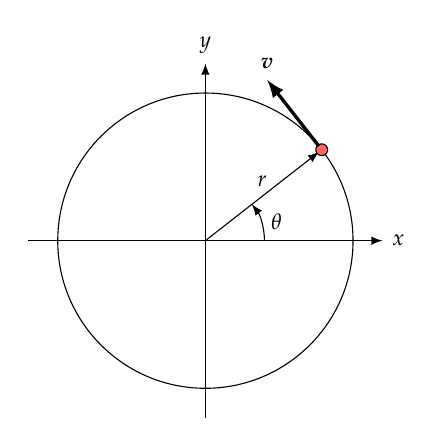
\begin{tikzpicture}[scale=.75]
      \draw[->](-3,0)--(3,0) node[right]{\footnotesize$x$};
      \draw[->](0,-3)--(0,3) node[above]{\footnotesize$y$};
      \draw (0,0) circle(2.5);
      \begin{scope}[rotate=38]
        \draw[->] (0,0)--(2.44,0) node[midway,above]{\footnotesize$r$};
        \draw[fill=red!60] (2.5,0) circle(.1);
        \draw[very thick,->](2.5,.08)--(2.5,1.5)
        node[above]{\footnotesize$\bm{v}$};
      \end{scope}
      \draw(1,0)[->] arc(0:38:1) node[midway,right]{\footnotesize$\theta$};
    \end{tikzpicture}

    \column{.7\textwidth}
    The velocity of the object in circular motion is more properly related to
    the angular velocity using this vector cross product:

    \eq{-.25in}{
      \bm{v}=\bm{\omega}\times\bm{r}
    }

    \begin{itemize}
    \item\vspace{-.2in}$\bm{\omega}$: out of the page if motion is
      counter-clockwise
    \item $\bm{\omega}$: into the page if motion is clockwise
    \end{itemize}
    Visualizing $\bm{\omega}$ takes practice, but this vector notation is
    mathematically rigorious and consistent
  \end{columns}
\end{frame}



\begin{frame}{Period \& Frequency}
  \begin{columns}
    \column{.3\textwidth}
    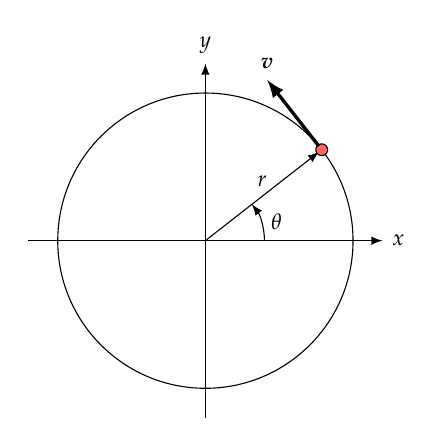
\begin{tikzpicture}[scale=.75]
      \draw[->](-3,0)--(3,0) node[right]{\footnotesize$x$};
      \draw[->](0,-3)--(0,3) node[above]{\footnotesize$y$};
      \draw (0,0) circle(2.5);
      \begin{scope}[rotate=38]
        \draw[->] (0,0)--(2.44,0) node[midway,above]{\footnotesize$r$};
        \draw[fill=red!60] (2.5,0) circle(.1);
        \draw[very thick,->](2.5,.08)--(2.5,1.5)
        node[above]{\footnotesize$\bm{v}$};
      \end{scope}
      \draw(1,0)[->] arc(0:38:1) node[midway,right]{\footnotesize$\theta$};
    \end{tikzpicture}

    \column{.7\textwidth}
    For constant angular velocity $\omega$ (uniform circular motion), the
    motion is periodic. Its \textbf{frequency} and \textbf{period} are given by:

    \eq{-.15in}{
      f=\frac{\omega}{2\pi}\quad
      T=\frac{2\pi}{\omega}\quad
      f=\frac1T
    }
    
    $T$ is in \textbf{seconds} (\si{\s}) and $f$ is in \textbf{hertz}
    (\si{\hertz})
  \end{columns}
\end{frame}



\begin{frame}{Rotating Object Without Slipping}
  A tire with radius $r$ rolls along the road with an angular velocity $\omega$
  \emph{without slipping}. (This is a very common case for analysis.)  What
  is its velocity $v$
  \begin{enumerate}[a.]
  \item at the contact between the ground and the tire?
  \item at the center?
  \item at the top of the tire?
  \end{enumerate}

  \vspace{-.4in}
  \begin{center}
    \hspace{1in}
    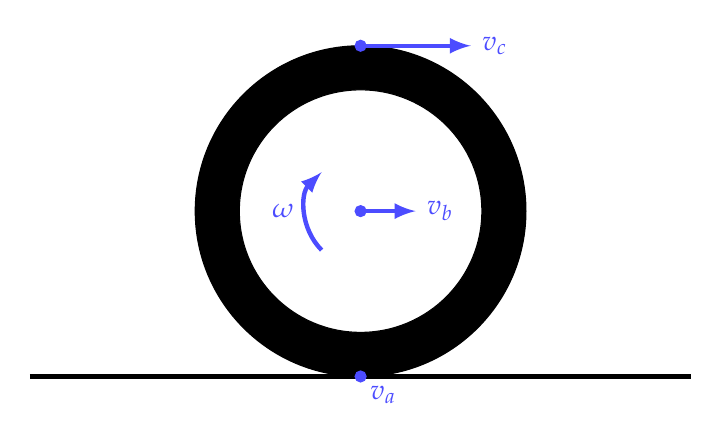
\begin{tikzpicture}[scale=.7]
      \draw[fill=black](0,0) circle(3);
      \draw[fill=white](0,0) circle(2.2);
      \draw[ultra thick](-6,-3)--(6,-3);
      \draw[ultra thick,blue!70,->](-.707,-.707) arc(225:135:1)
      node[midway,left]{$\omega$};
      \draw[fill=blue!70,blue!70](0,-3) circle(.1) node[below right]{$v_a$};
      \draw[fill=blue!70,blue!70](0,0) circle(.1);
      \draw[ultra thick,blue!70,->](0,0)--(1,0) node[right]{$v_b$};
      \draw[fill=blue!70,blue!70](0,3) circle(.1);
      \draw[ultra thick,blue!70,->](0,3)--(2,3) node[right]{$v_c$};
    \end{tikzpicture}
  \end{center}
\end{frame}



\begin{frame}{Angular Acceleration}
  The time derivative of $\omega$ is \textbf{angular acceleration}, which
  has a unit of \si{rad/\second^2}:

  \eq{-.2in}{
    \alpha=\dot{\omega}=\ddot{\theta}
  }

  Similar to the relationship between velocity and angular velocity,
  \textbf{tangential acceleration} $a_t$ is related to angular acceleration
  $\alpha$ by the radius $r$:
    
  \eq{-.2in}{
    a_t(t)=\dot{v}=r\dot{\omega}=r\alpha
  }
    
  For \emph{uniform} circular motion, $\omega$ is constant, and therefore
  $a_t=0$
\end{frame}



\begin{frame}{With Calculus}
  Relationship between angular position and angular velocity:

  \eq{-.2in}{
    \omega(t)=\frac{d\theta}{dt}\quad\quad
    \theta(t)=\int\omega(t) dt +\theta_0
  }

  Relationship between angular velocity and angular acceleration:

  \eq{-.2in}{
    \alpha(t)=\frac{d\omega}{dt}=\frac{d^2\theta}{dt^2}
    \quad\quad\omega(t)=\int\alpha(t) dt+\omega_0
  }

  The relationships are the same as in rectilinear motion.
\end{frame}




\begin{frame}{Kinematics in the Angular Direction}
  For constant $\alpha$, the kinematic equations are just like in rectilinear
  motion:

  \vspace{-.3in}{\Large
    \begin{align*}
      \theta&=\theta_0 + \omega_0 t + \frac{1}{2}\alpha t^2\\
      \theta&=\theta_0+ \frac{\omega_0+\omega}{2} t\\
      \omega^2& = \omega_0^2+ 2\alpha(\theta-\theta_0)
    \end{align*}
  }
  
  If $\alpha$ is \emph{not} constant, integration will be required.
\end{frame}



\begin{frame}{A Simple Example}
  \textbf{Example 1:} An object moves in a circle with angular acceleration
  \SI{3.}{rad/\s^2}. The radius is \SI{2.}{\metre} and it starts from rest. How
  long does it take for this object to finish a circle?
\end{frame}



\begin{frame}{Centripetal Acceleration \& Centripetal Force}
  There is also a component of acceleration toward the center of the motion,
  called the \textbf{centripetal acceleration} $a_c$:

  \eq{-.15in}{
    \boxed{\bm{a}_c=-\frac{v^2}{r}\hat{\bm{r}}=-(\omega^2r)\hat{\bm{r}}}
  }

  (The negative sign is because $\hat{\bm{r}}$ is radially outward from the
  center.) The force that causes the centripetal acceleration is called the
  \textbf{centripetal force}:

  \eq{-.15in}{
    \boxed{\bm{F}_c=m\bm{a}_c=-\frac{mv^2}{r}\hat{\bm{r}}}
  }
\end{frame}



\begin{frame}{Centripetal Acceleration for Uniform Circular Motion}
  In uniform circular motion ($\alpha=0$) problems where the period or
  frequency are known, the speed of the object is:

  \eq{-.15in}{
    %v=\frac{2\pi r}{T}=2\pi rf
    v=\omega r = 2\pi rf = \frac{2\pi r}T
  }

  Centripetal acceleration can therefore be expressed based on $T$ or $f$:

  \eq{-.2in}{
    \bm{a}_c=-\frac{v^2}{r}\hat{\bm{r}}\quad\rightarrow\quad
    \boxed{
      \bm{a}_c=-\frac{4\pi^2r}{T^2}\hat{\bm{r}}=-4\pi^2rf^2\hat{\bm{r}}
    }
  }
\end{frame}



\begin{frame}{Acceleration: The General Case}
  \begin{columns}
    \column{.25\textwidth}
    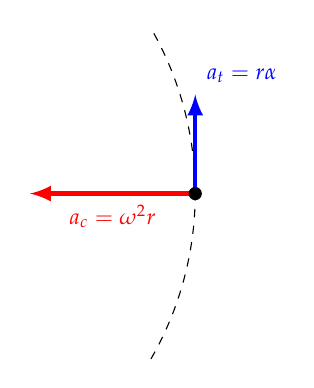
\begin{tikzpicture}[scale=4.2]
      \draw[dashed] (.866,-.5) arc(-30:30:1);
      \draw[ultra thick,red,->] (1,0)--(.5,0)
      node[midway,below]{\footnotesize $a_c=\omega^2r$};
      \draw[ultra thick, blue,->] (1,0)--(1,.3)
      node[above right]{\footnotesize $a_t=r\alpha$};
      \fill (1,0) circle(.02);
    \end{tikzpicture}
    
    \column{.75\textwidth}
    In general circular motion, there are two components of acceleration:
    \begin{itemize}
    \item\textcolor{red}{\textbf{Centripetal acceleration} $a_c$} depends on
      radius of curvature $r$ and instantaneous speed $v$. The direction of
      the acceleration is toward the center of the circle.
    \item \textcolor{blue}{\textbf{Tangential acceleration} $a_t$}
      depends on radius $r$  and angular acceleration $\alpha$. The direction
      of the acceleration is tangent to the circle
    \end{itemize}
  \end{columns}

  \vspace{.2in}Most of the cases in AP Physics are uniform circular motion.
\end{frame}



\begin{frame}{How to Solve Circular Motion Problems}
  The condition for circular motion is the second law of motion:

  \eq{-.2in}{
    \bm{F}_c=\sum\bm{F}=m\bm{a}_c
  }
  
  The forces that generate the centripetal force comes from the free-body
  diagram. It may include:
  \begin{itemize}
  \item Gravity
  \item Friction
  \item Normal force
  \item Tension
  \item Etc.
  \end{itemize}
\end{frame}



\begin{frame}{Example: Horizontal Motion}
  \begin{columns}
    \column{.4\textwidth}
    \pic{1}{puck-on-table.png}
    
    \column{.6\textwidth}
    \textbf{Example 2:} In the figure on the left, a mass
    $m_1=\SI{3.}{\kilo\gram}$ is rolling around a frictionless table with
    radius $R=\SI{1.}{\metre}$. with a speed of \SI{2.}{\metre\per\second}.
    What is the mass of the weight $m_2$?
  \end{columns}
\end{frame}



\begin{frame}{Banked Curves on Highways and Racetracks}
  \begin{columns}
    \column{.35\textwidth}
    \centering
    \pic{.8}{banked-turn-acceleration.png}\\
    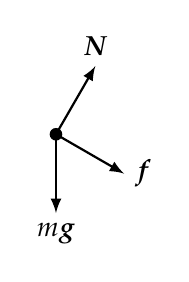
\begin{tikzpicture}
      \fill[black](0,0) circle(.08);
      \draw[thick,->,rotate=-30](0,0)--(0,1)node[above]{$\bm{N}$};
      \draw[thick,->](0,0)--(0,-1)node[below]{$m\bm{g}$};
      \draw[thick,->,rotate=60](0,0)--(0,-1)node[right]{$\bm{f}$};
    \end{tikzpicture}
    \begin{tikzpicture}
      \draw[->](0,0)--(1,0) node[right]{$x$};
      \draw[->](0,0)--(0,1) node[above]{$y$};
    \end{tikzpicture}

    \column{.65\textwidth}
    No motion in the $y$ direction, i.e.\ no net force:

    \eq{-.35in}{
      \sum F_y=N\cos\theta-f\sin\theta-w=0
    }

    Net force in the $x$ direction is the centripetal force:

    \eq{-.35in}{
      \sum F_x=N\sin\theta +f\cos\theta = \frac{mv^2}{r}
    }

    Friction force $\bm{f}$ may be static or kinetic.
  \end{columns}
\end{frame}



\begin{frame}{Banked Curves on Highways and Racetracks}
  \begin{columns}
    \column{.35\textwidth}
    \centering
    \pic{.8}{banked-turn-acceleration.png}\\
    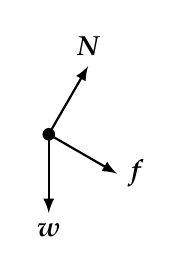
\begin{tikzpicture}
      \fill[black](0,0) circle(.08);
      \draw[thick,->,rotate=-30](0,0)--(0,1)node[above]{$\bm{N}$};
      \draw[thick,->](0,0)--(0,-1)node[below]{$\bm{w}$};
      \draw[thick,->,rotate=60](0,0)--(0,-1)node[right]{$\bm{f}$};
    \end{tikzpicture}
    \begin{tikzpicture}
      \draw[->](0,0)--(1,0) node[right]{$x$};
      \draw[->](0,0)--(0,1) node[above]{$y$};
    \end{tikzpicture}

    \column{.65\textwidth}
    For analysis, use the simplified equation for friction $f=\mu N$ (i.e.\
    assume either kinetic friction or maximum static friction), and weight
    $w=mg$, the equations on the previous slides can be arranged as:

    \vspace{-.4in}{\Large
      \begin{align*}
        N\left(\cos\theta-\mu\sin\theta\right) &=mg\\
        N\left(\sin\theta+\mu\cos\theta\right) &=\frac{mv^2}{r}
      \end{align*}
    }
  \end{columns}
\end{frame}


\begin{frame}{Banked Curves on Highways and Racetracks}
  \begin{columns}
    \column{.35\textwidth}
    \centering
    \pic{.8}{banked-turn-acceleration.png}\\
    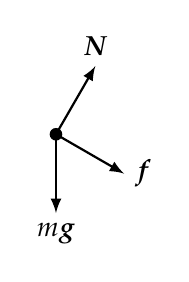
\begin{tikzpicture}
      \fill[black](0,0) circle(.08);
      \draw[thick,->,rotate=-30](0,0)--(0,1)node[above]{$\bm{N}$};
      \draw[thick,->](0,0)--(0,-1)node[below]{$m\bm{g}$};
      \draw[thick,->,rotate=60](0,0)--(0,-1)node[right]{$\bm{f}$};
    \end{tikzpicture}
    \begin{tikzpicture}
      \draw[->](0,0)--(1,0) node[right]{$x$};
      \draw[->](0,0)--(0,1) node[above]{$y$};
    \end{tikzpicture}

    \column{.65\textwidth}
    Dividing the two equations removes both the normal force and mass terms:

    \eq{-.15in}{
      \frac{\sin\theta+\mu\cos\theta}{\cos\theta-\mu\sin\theta}
      =\frac{v^2}{rg}
    }

    The \emph{maximum} velocity $v_\text{max}$ can be expressed as:

    \eq{-.25in}{
      \boxed{v_\text{max}=
        \sqrt{rg\frac{\sin\theta+\mu\cos\theta}{\cos\theta-\mu\sin\theta}}
      }
    }

    Note that $v_\text{max}$ does not depend on mass.
  \end{columns}
\end{frame}



\begin{frame}{Banked Curves on Highways and Racetracks}
  In the limit of $\mu=0$ (frictionless case), the equation reduces to:

  \eq{-.1in}{
    \boxed{ v_{\text{max}}=\sqrt{rg\tan\theta} }
  }

  And in the limit of a flat roadway with no banking ($\theta=0$,
  $\sin\theta=0$ and $\cos\theta=1$), the equation reduces to:

  \eq{-.2in}{
    \boxed{
      v_{\text{max}}=\sqrt{\mu rg}
    }
  }
\end{frame}




%
%
%\begin{frame}{Another Example: Exit Ramp}
%  \textbf{Example 3:} A car exits a highway on a ramp that is banked at
%  \ang{15} to the horizontal. The exit ramp has a radius of curvature of
%  \SI{65}{\metre}. If the conditions are extremely icy and the driver cannot
%  depend on any friction to help make the turn, at what speed should the driver
%  travel so that the car will not skid off the ramp? What if there is friction?
%\end{frame}


\section{Vertical Circles}

\begin{frame}{Vertical Circles}
  Circular motion with a horizontal path is straightforward. However, for
  vertical motion:
  \begin{itemize}
  \item Generally difficult to solve by dynamics and kinematics
  \item Instead, use conservation of energy to solve for $\bm{v}$
  \item Then use the equation for centripetal force to find other forces
  \end{itemize}

  \textbf{Remember:} If it is impossible to get the required centripetal
  force, then it could not continue the circular motion
\end{frame}



\begin{frame}{What About a Pendulum?}
  A simple pendulum is also like a vertical circular motion problem.

  \vspace{.1in}\begin{columns}
    \column{.35\textwidth}
    \begin{tikzpicture}[scale=.8]
      \fill[pattern=north east lines] (-1,0) rectangle (1,0.2);
      \draw[very thick](-1,0)--(1,0);
      \begin{scope}[rotate=20]
        \draw[thick](0,0)--(0,-5);
        \tikzstyle{balloon}=[ball color=red!70!black];
        \shade[balloon] (0,-5) circle (0.2) node[below right]{$m$};
        \begin{scope}[->,very thick,red!70!black]
          \draw(0,-5)--(0,-3.3) node[left]{\footnotesize $\bm{T}$};
          \draw[rotate around={-20:(0,-5)}](0,-5)--(0,-6.5)
          node[below]{\footnotesize $m\bm{g}$};
        \end{scope}
      \end{scope}
      \draw[dashed,thin](0,0)--(0,-5);
      \draw[dashed,thin](3.54,-3.54) arc(315:225:5);
      \draw[->](0,-2) arc(270:290:2) node[midway,below]{$\theta$};
    \end{tikzpicture}

    \column{.65\textwidth}
    \begin{itemize}
    \item There are two forces act on the pendulum: weight $\bm{w}=m\bm{g}$, and
    tension $\bm{T}$
    \item Speed of the pendulum at any height is found using conservation
      of energy
      \begin{itemize}
      \item Tension $\bm{T}$ is always $\perp$ to motion, therefore it doesn't
        do any work
      \item Work is done by gravity (a conservative force) alone
      \end{itemize}
    %\item The velocity vector is tangent to the path
    \item Tangential and centripetal accelerations are based on the net force
      along the angular and radial directions
    \end{itemize}
  \end{columns}
\end{frame}



\begin{frame}{Simple Pendulum}
  At the top of the swing, velocity $v$ is zero, therefore:
  
  \vspace{.1in}\begin{columns}
    \column{.5\textwidth}
    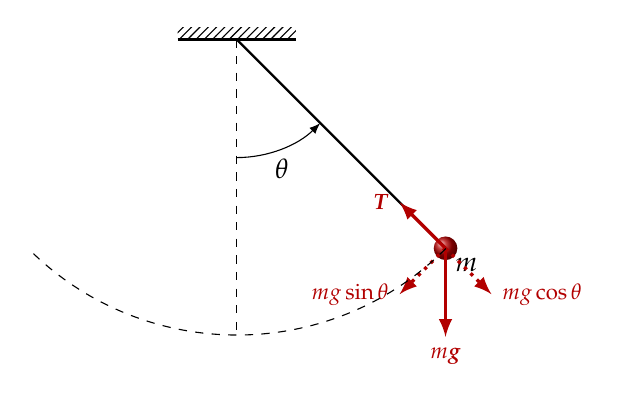
\begin{tikzpicture}[scale=.75]
      \fill[pattern=north east lines] (-1,0) rectangle (1,0.2);
      \draw[very thick](-1,0)--(1,0);
      \begin{scope}[rotate=45]
        \draw[thick](0,0)--(0,-5);
        \tikzstyle{balloon}=[ball color=red!70!black];    
        \shade[balloon] (0,-5) circle (0.2) node[below right]{$m$};
        \begin{scope}[->,very thick,red!70!black]
          \draw[dotted](0,-5)--(-1.1,-5)node[left]{\footnotesize$mg\sin\theta$};
          \draw[dotted](0,-5)--(0,-6.1)node[right]{\footnotesize$mg\cos\theta$};
          \draw(0,-5)--(0,-3.9) node[left]{\footnotesize $\bm{T}$};
          \draw[rotate around={-45:(0,-5)}](0,-5)--(0,-6.5)
          node[below]{\footnotesize $m\bm{g}$};
        \end{scope}
      \end{scope}
      \draw[dashed,thin](0,0)--(0,-5);
      \draw[dashed,thin](3.54,-3.54) arc(315:225:5);
      \draw[->](0,-2) arc(270:315:2) node[pos=.5,below]{$\theta$};
    \end{tikzpicture}

    \column{.5\textwidth}
    Centripetal acceleration is also zero:

    \eq{-.2in}{
      a_c=\frac{v^2}{r}=0
    }

    and therefore the net force along the radial direction $\hat{\bm{r}}$ is
    zero. The tension force $T$ can be calculated:

    \eq{-.2in}{
      T=mg\cos\theta
    }
  \end{columns}
  At the highest point when $\theta$ is largest, tension is the lowest.
\end{frame}



\begin{frame}{Simple Pendulum}
  In the radial direction $\hat{\bm{\theta}}$, there is still a net force of
  $mg\sin\theta$, therefore:
  \begin{columns}
    \column{.5\textwidth}
    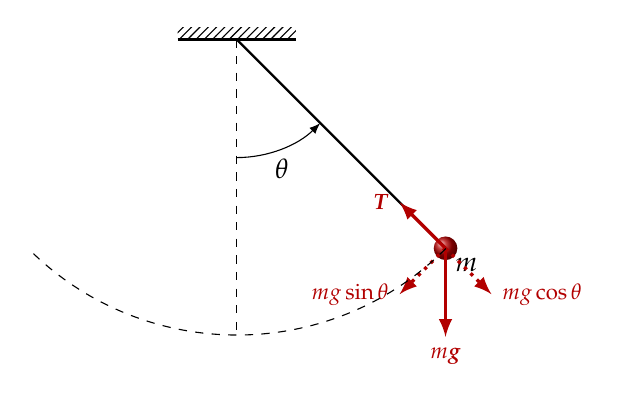
\begin{tikzpicture}[scale=.75]
      \fill[pattern=north east lines] (-1,0) rectangle (1,0.2);
      \draw[very thick](-1,0)--(1,0);
      \begin{scope}[rotate=45]
        \draw[thick](0,0)--(0,-5);
        \tikzstyle{balloon}=[ball color=red!70!black];    
        \shade[balloon] (0,-5) circle (0.2) node[below right]{$m$};
        \draw[dotted,->,very thick,red!70!black](0,-5)--(-1.1,-5)
        node[left]{\footnotesize $mg\sin\theta$};
        \draw[dotted,->,very thick,red!70!black](0,-5)--(0,-6.1)
        node[right]{\footnotesize $mg\cos\theta$};
        \draw[->,very thick,red!70!black](0,-5)--(0,-3.9)
        node[left]{\footnotesize $\bm{T}$};
        \draw[->,very thick,red!70!black,rotate around={-45:(0,-5)}]
        (0,-5)--(0,-6.5) node[below]{\footnotesize $m\bm{g}$};
      \end{scope}
      \draw[dashed,thin](0,0)--(0,-5);
      \draw[dashed,thin](3.54,-3.54) arc(315:225:5);
      \draw[->](0,-2) arc(270:315:2) node[pos=.5,below]{$\theta$};
    \end{tikzpicture}

    \column{.5\textwidth}
    There is a tengential acceleration along $\hat{\bm{\theta}}$, with a
    magnitude of:

    \eq{-.25in}{
      a_t=g\sin\theta
    }

    \vspace{-.1in}This is the same acceleration as an object sliding down a
    frictionless ramp at an angle of $\theta$.
  \end{columns}
\end{frame}



\begin{frame}{Simple Pendulum}
  At the bottom of the swing, the velocity is at its maximum value,
  
  \vspace{.1in}\begin{columns}
    \column{.35\textwidth}
    \begin{tikzpicture}[scale=.8]
      \fill[pattern=north east lines] (-1,0) rectangle (1,0.2);
      \draw[very thick](-1,0)--(1,0);

      \draw[thick](0,0)--(0,-5);
      \tikzstyle{balloon}=[ball color=red!70!black];    
      \shade[balloon] (0,-5) circle (0.2) node[below right]{$m$};
      \begin{scope}[->,very thick,red!70!black]
        \draw (0,-5)--(0,-2.5) node[right]{\footnotesize $\bm{T}$};
        \draw (0,-5)--(0,-6.5) node[below]{\footnotesize $m\bm{g}$};
      \end{scope}
      \draw[dashed,thin](0,0)--(0,-5);
      \draw[dashed,thin](3.54,-3.54) arc(315:225:5);
    \end{tikzpicture}

    \column{.65\textwidth}
    \begin{itemize}
    \item Maximum centripetal acceleration:

      \eq{-.25in}{
        a_c=\frac{v^2}r
      }
    \item No tangential acceleration:

      \eq{-.25in}{
        a_t=0
      }
    \item At the lowest point, tension is the highest:

      \eq{-.3in}{
        T=w+F_c=m\left(g+\frac{v^2}{r}\right)
      }
    \end{itemize}
  \end{columns}
\end{frame}



\begin{frame}{Example Problem}
  \textbf{Example 4:} You are playing with a yo-yo with a mass of
  \SI{225}{\gram}. The full length of the string is \SI{1.2}{\metre}. You
  decide to see how slowly you can swing it in a vertical circle while keeping
  the string fully extended, even when the yo-yo is at the top of its swing.
  \begin{enumerate}[A.]
  \item Calculate the minimum speed at which you can swing the yo-yo while
    keeping it on a circular path.
  \item Find the tension in the string when the yo-yo is at the side and at the
    bottom of its swing. 
  \end{enumerate}
\end{frame}



\begin{frame}{Example Problem}
  \textbf{Example 5:} A cord is tied to a pail of water, and the pail is swung
  in a vertical circle of \SI{1.}{\metre}. What must be the minimum velocity of
  the pail be at its highest point so that no water spills out?

  \begin{enumerate}[(a)]
  \item\SI{3.1}{\metre\per\second}
  \item\SI{5.6}{\metre\per\second}
  \item\SI{20.7}{\metre\per\second}
  \item\SI{100.5}{\metre\per\second}
  \end{enumerate}
\end{frame}



\begin{frame}{Example: Roller Coaster}
  \textbf{Example 6:} A roller coaster car is on a track that forms a circular
  loop, of radius $R$, in the vertical plane. If the car is to maintain contact
  with the track at the top of the loop (generally considered to be a good
  thing), what is the minimum speed that the car must have at the bottom of the
  loop. Ignore air resistance and rolling friction.
  \begin{enumerate}[(a)]
  \item $\sqrt{2gR}$
  \item $\sqrt{3gR}$
  \item $\sqrt{4gR}$
  \item $\sqrt{5gR}$
  \end{enumerate}
\end{frame}



\begin{frame}{Example}
  \textbf{Example 7:} A stone of mass $m$ is attached to a light strong string
  and whirled in a \emph{vertical} circle of radius $r$. At the exact bottom of
  the path, the tension of the string is three times the weight of the stone.
  The stone's speed at that point is given by:
  \begin{enumerate}[(a)]
  \item $2\sqrt{gR}$
  \item $\sqrt{2gR}$
  \item $\sqrt{3gR}$
  \item $4gR$
  \end{enumerate}
\end{frame}
\end{document}
